%%%%%%%%%%%%%%%%%%%% author.tex %%%%%%%%%%%%%%%%%%%%%%%%%%%%%%%%%%%
%
% sample root file for your "contribution" to a contributed volume
%
% Use this file as a template for your own input.
%
%%%%%%%%%%%%%%%% Springer %%%%%%%%%%%%%%%%%%%%%%%%%%%%%%%%%%%%%%%%%


%% RECOMMENDED %%%%%%%%%%%%%%%%%%%%%%%%%%%%%%%%%%%%%%%%%%%%%%%%%%%
%\documentclass[graybox]{svmult}
%
%% choose options for [] as required from the list
%% in the Reference Guide
%
%\usepackage{mathptmx}       % selects Times Roman as basic font
%\usepackage{helvet}         % selects Helvetica as sans-serif font
%\usepackage{courier}        % selects Courier as typewriter font
%\usepackage{type1cm}        % activate if the above 3 fonts are
                             % not available on your system
%
%\usepackage{makeidx}         % allows index generation
%\usepackage{graphicx}        % standard LaTeX graphics tool
%                             % when including figure files
%\usepackage{multicol}        % used for the two-column index
%\usepackage[bottom]{footmisc}% places footnotes at page bottom
%
%% see the list of further useful packages
%% in the Reference Guide
%
%\makeindex             % used for the subject index
%                       % please use the style svind.ist with
%                       % your makeindex program
%
%%%%%%%%%%%%%%%%%%%%%%%%%%%%%%%%%%%%%%%%%%%%%%%%%%%%%%%%%%%%%%%%%%%%%%%%%%%%%%%%%%%%%%%%%%
%
%\begin{document}

\title{Tropical Cyclone - Storm Surge}
% Use \titlerunning{Short Title} for an abbreviated version of
% your contribution title if the original one is too long
\author{
    \textbf{Andrew Kennedy} 
    \and {George Deodatis}
    \and {Ajay Harish}
    \and {Rick Luettich}
    \and {Lance Manuel}}
\tocauthor{}
\authorrunning{Andrew Kennedy et al.}
% Use \authorrunning{Short Title} for an abbreviated version of
% your contribution title if the original one is too long
%\institute{Name of First Author \at Name, Address of Institute, %\email{name@email.address}
%\and Name of Second Author \at Name, Address of Institute %\email{name@email.address}}
%
% Use the package "url.sty" to avoid
% problems with special characters
% used in your e-mail or web address
%
\maketitle

Simulations of coastal storm surge are used for planning, forecasting, nowcasting, hindcasting, climatological studies, and risk evaluation; the need for surge studies has been continual over recent years and there is an ongoing need for trained professionals. The largest surges occur from tropical cyclones, but strong winter storms may also generate high water levels.

Surge studies are in many ways broadly similar: a wind and pressure field forces a hydrodynamic model, potentially inundating areas of interest. Details of modeling differ, with numerics, resolution, bottom friction, and theoretical assumptions as noticeable differences. Some systems include additional components such as wave setup and runup, while these are neglected by others. Atmospheric forcing can either be raster-based, where large-scale wind and pressure fields force the modeling system, or may arise from a tropical or extratropical storm scenario described by a storm track and set of parameters describing strength and size. These simulations yield geospatially distributed estimates of storm surge (storm-induced rise in seawater levels, primarily caused by wind) for the purposes of direct and indirect loss assessment for coastal communities \citep{jacobResponding2011}. Estimates of storm-induced inundation, due to combined effects of storm surge and waves driving water over land, are important outputs from any simulation environment that help quantify damage to structures as well as above and below ground civil infrastructure.

Because surge models can be expensive, in general there is a need to manage the tradeoff between model fidelity and computational efficiency. One method that has seen increasing adoption in recent years uses surrogate models. Given a database of high-fidelity model runs to be used as a training set, surrogate models can reduce CPU times of model runs from hundreds and even thousands of hours to minutes and enable computationally efficient means to characterize uncertainty in the hazard (e.g., the hurricane track) for the purposes of risk assessment \citep{kijewski-correaCyberEye2014}. However, these require large-scale training sets that may not be straightforward to generate. 

\section{Common Modeling Approaches}
\label{sec:storm_surge_methods}

This section examines the three classes of models commonly coupled to capture storm surge and accompanying wave effects nearshore and overland, as well as surrogate models that can be tailored to these coupled models for a computationally efficient simulation alternative. Note: this is not an exhaustive presentation of the simulation tools available for coastal hazards but focuses only on those viewed as the industry standard. 

\subsection{Storm surge heights and inundation}

Numerical models for storm-surge simulations are typically based on single-layer (or sometimes multi-layer) depth averaged shallow water equations describing fluid motion driven by storm winds and pressure. These simplifications are necessary as a full Navier-Stokes based approach is computationally infeasible. The available numerical models differ in their computational solution strategies, with implications for the spatial and temporal resolution of the simulations, the required computational resources and runtimes, and the required input data and model parameters. Generally, these models capture the amplitude of long-period, long-gravity waves and do not simulate short-period wave effects, which are addressed in subsequent sections. Models may be distinguished by resolution, numerics, assumptions, and computational efficiency. Models described here are:

\begin{enumerate}
    \item Sea, Lake and Overland Surges from Hurricanes  (SLOSH)
    \item ADvanced CIRCulation model (ADCIRC)
    \item Delft3D 
    \item Finite Volume COMmunity Model (FVCOM)
    \item GeoClaw
\end{enumerate}

\noindent\textbf{SLOSH} \\The National Weather Service (NWS) utilizes a storm-surge model called Sea, Lake and Overland Surges from Hurricanes (SLOSH), which solves the shallow water equations using structured curvilinear grids (Jelesnianski et al., 1992). It was developed to provide real-time estimates of storm surge on a single computational core; therefore, the grid resolution and the resulting spatial resolution of the results are fairly coarse. As reported by Mandli and Dawson (2014), a primary limitation of SLOSH is “the limited domain size and extents allowed due to the grid mapping used and formulation of the equations.” Nevertheless, since its initial development, SLOSH has continued to be updated and is used for real-time forecasts of surge for public advisories and to inform emergency responders. SLOSH is very computationally efficient, and this allows it to perform probabilistic simulations of storm surge prior to a hurricane landfall using several thousand runs to obtain some measures of the potential surge if storm tracks and intensities change. Because SLOSH has been used for many years and does not contain all modern features, it may at some point be transitioned to a different model, the most likely being the Coastal and Estuarine Storm Tide model (CEST) \citep{zhangTransition2017}. 
\newline

\noindent\textbf{ADCIRC} \\The ADvanced CIRCulation (ADCIRC) methodology is commonly regarded as the state-of-the-art in high resolution coastal storm-surge simulation \citep{luettichADCIRC1992}, capable of providing significantly more accurate simulations than methods based on SLOSH \citep{resioModeling2008} in near-shore coastal regions. As such, ADCIRC is the preferred methodology for coastal storm-surge investigations by the U.S. Army Corps of Engineers (USACE) and is one of the two models certified for the generation of FEMA Digital Flood Insurance Rate Maps (DFIRMSs). ADCIRC solves the depth-averaged shallow water equations describing on a rotating earth, formulated using the traditional hydrostatic pressure and Boussinesq approximations, and discretized in space using the finite-element method and in time using the finite-difference method. ADCIRC can be run either as a 2D depth integrated (2DDI) model or as a 3D model, with elevation resulting from the solution of the depth-integrated continuity equation in generalized wave-continuity equation (GWCE) form. Furthermore, velocity is obtained from the solution of either the 2DDI or 3D momentum equations, retaining all nonlinear terms. ADCIRC simulations have been validated for major hurricanes such as Katrina, Ike, Gustav, and Iniki \citep{kennedyOrigin2011,kennedyTropical2012}. ADCIRC has been parallelized efficiently, with linear speedups to hundreds or thousands of cores for large domains. 
\newline

\noindent\textbf{Delft3D} \\Delft3D-Flow is the second model certified for FEMA DFIRM generation. It is based on shallow water equations in either depth-averaged or multi-layer formulation, and is used widely among engineering consultants and researchers \citep{huNumerical2015,vousdoukasProjections2016}. Delft3D may be run in either serial or parallel modes, with typical parallel runs using tens of cores. The Delft3D-Flow surge model is a part of a larger suite of interrelated models that include spectral wave, and coastal runup/morphological evolution \cite{deltaressystemsDelft3D2011}. 
\newline

\noindent\textbf{FVCOM} \\FVCOM is s finite volume-based model that has been used by numerous academic researchers to study storm surge \citep{kerrIOOS2013,regoStorm2010}. It is based on unstructured meshes, and shows similar skill to other models when run on a similar grid. The use of FVCOM for storm surge studies is in some ways a simplification of the full model, which includes momentum, continuity, temperature, salinity and density. It was originally developed for coastal and estuarine circulation by the oceanographical community, and is fully open source \citep{chenUnstructured2003}. 
\newline

\noindent\textbf{GEOCLAW} \\GEOCLAW, the final computational platform, lies between SLOSH and ADCIRC in terms of modeling resolution and computational cost. Originally developed to simulate tsunami inundation, GEOCLAW has recently been adapted to simulate storm surge (Berger et al., 2011, Mandli et al., 2014). Based on the CLAWPACK software libraries (LeVeque, 2002), GEOCLAW is an open-source, finite-volume, wave-propagation numerical model used to estimate hurricane-induced storm surge along a coastline. For overland flooding, the model uses Manning's n to parameterize roughness due to objects such as trees and small-scale structures that cannot be resolved computationally. Adaptive mesh refinement allows GEOCLAW to place computational resources where and when they are needed during a simulation. Thus, the overall cost of the simulation is reduced, while retaining the same or similar accuracy characteristics to ADCIRC. Shown in Figure \ref{fig:GEOCLAW_ADCIRC_comparison} is a comparison of results calculated using GEOCLAW versus ADCIRC. 

\begin{figure}[htb]
    \centering
    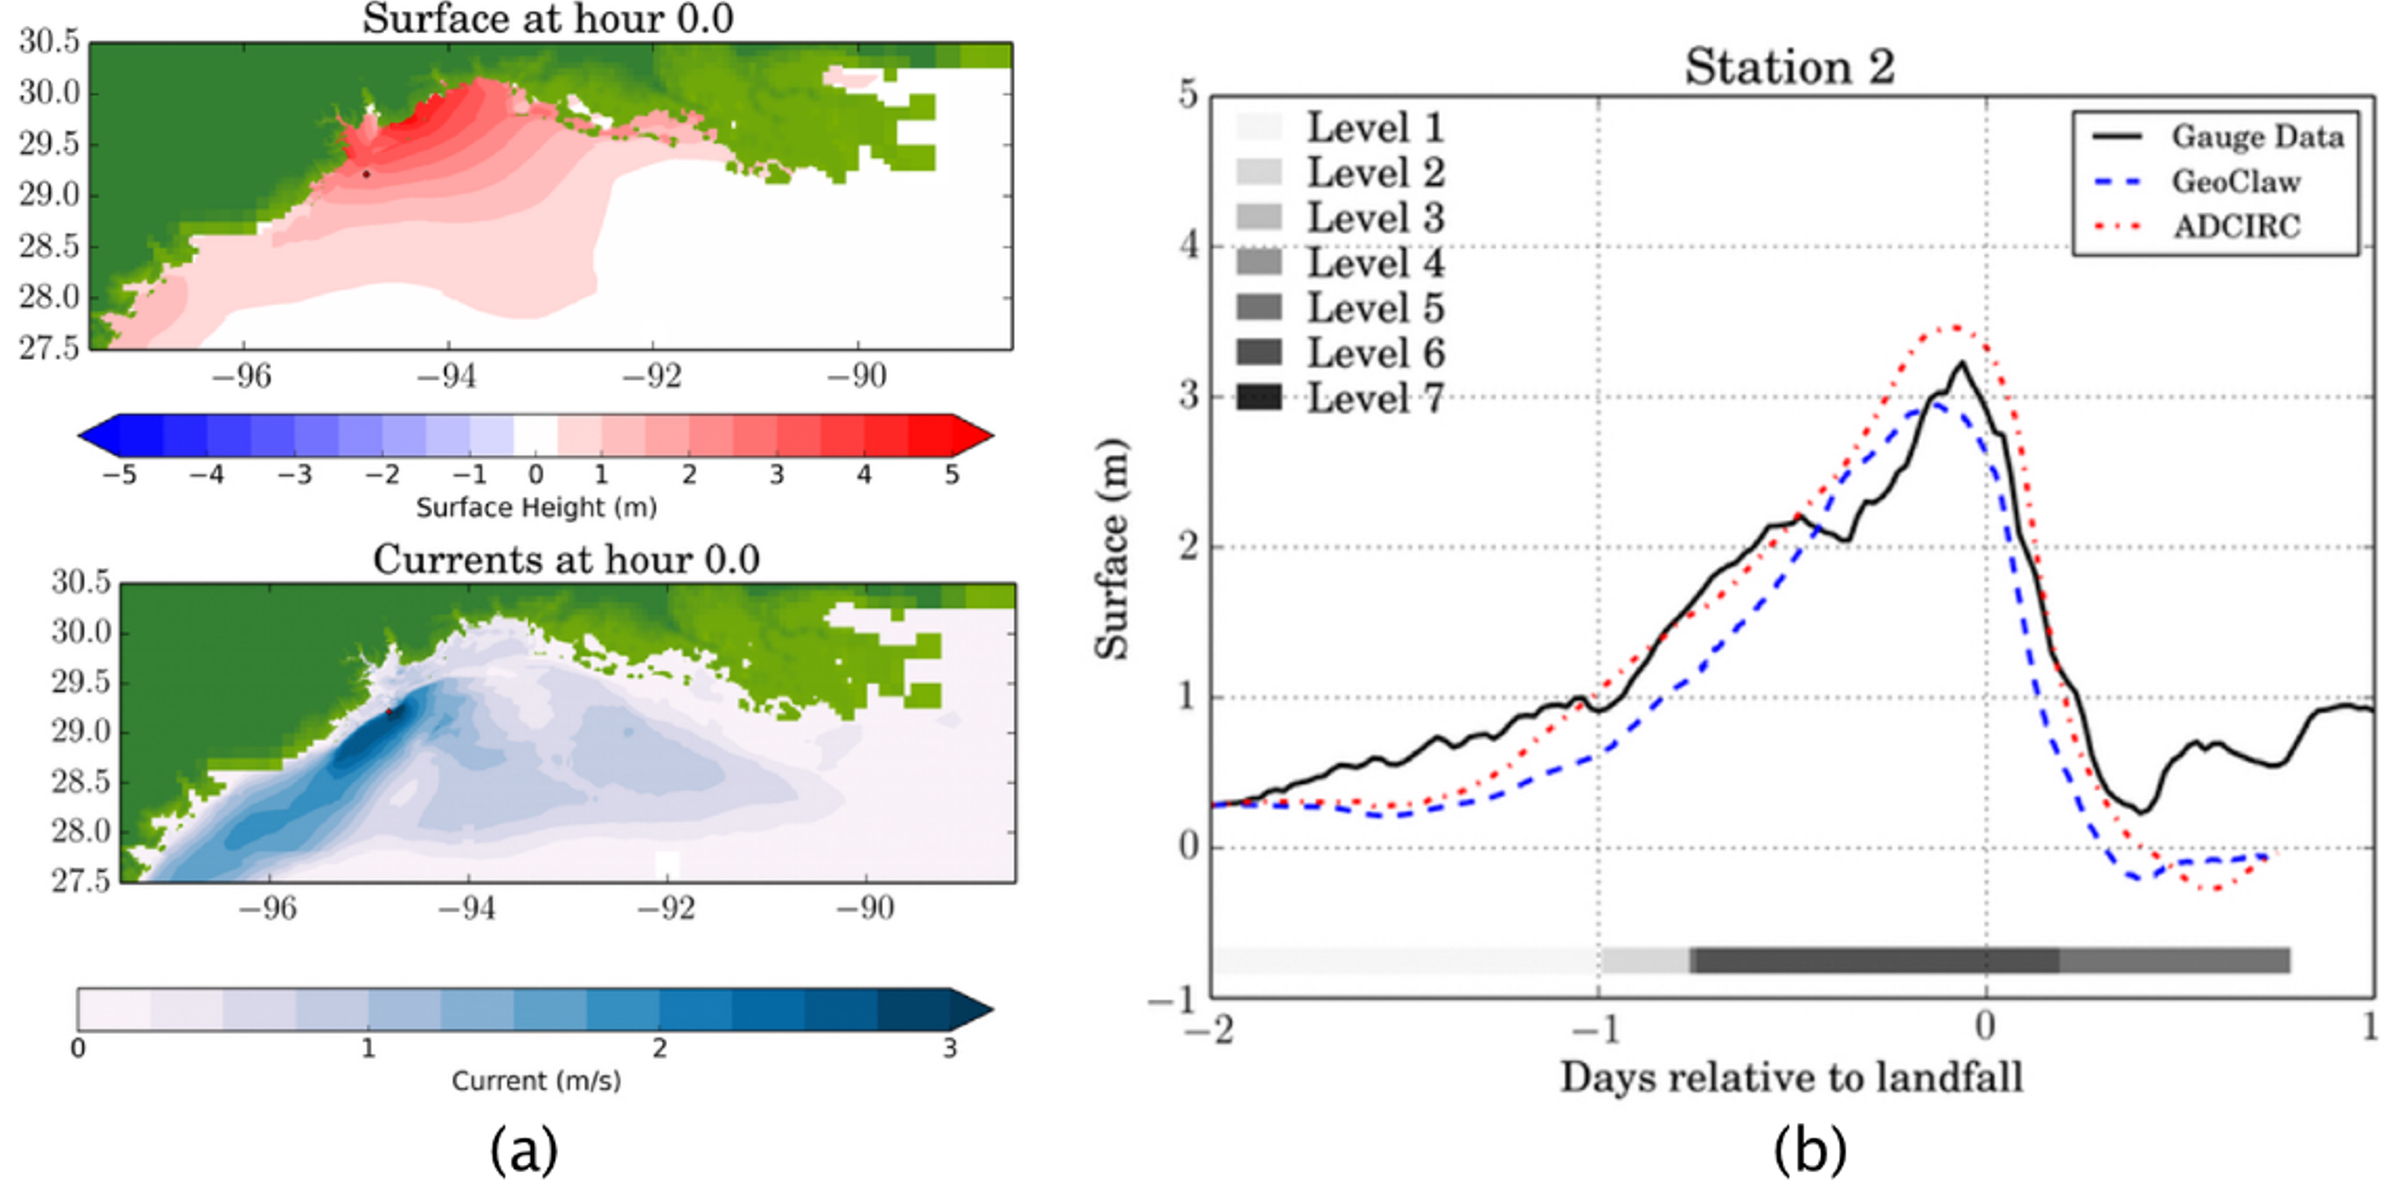
\includegraphics[width=1.0\textwidth, angle = 0]{Figures/GEOCLAW_ADCIRC_comparison.png}
    \caption{(a) A snapshot of a GEOCLAW storm surge simulation of Hurricane Ike at landfall; and (b) tide gauge data computed from GEOCLAW and ADCIRC along with observed data at the same location. \citep{mandli2016a}}
    \label{fig:GEOCLAW_ADCIRC_comparison}
\end{figure}

\subsection{Spectral wave models}

The platforms described above simulate slowly-varying surge heights but do not capture local wave effects. To do this, requires a separate wave model, either run as a fully-coupled system where both models pass information to each other, or as a one-way loosely coupled system. In two-way coupling, wave models pass radiation stresses to the surge model, while the surge model passes water levels and currents to the wave model. In one-way coupling, which is less accurate, the wave model is run at some given water level and radiation stresses are passed to the surge model.

The most common model used is Simulating WAves Nearshore (SWAN), which solves equations for wave spectral density in both frequency and direction \citep{zijlema2010a}. ADCIRC has been coupled previously with SWAN \citep{dietrich2011a,kennedyTropical2012}. The most recent North Atlantic Coastal Comprehensive Study (NACCS) (USACE 2015) employs STWAVE, which is a steady-state, finite difference spectral model for nearshore wind-wave growth and propagation based on the wave action balance equation (Smith et al., 2001). STWAVE simulates depth-induced wave refraction and shoaling, current-induced refraction and shoaling, depth- and steepness-induced wave breaking, diffraction, wave growth because of wind input, and wave–wave interaction and white capping that redistributes and dissipates energy in a growing wave field. Figure \ref{fig:surge_validation} validates the coupled hydrodynamic models used in the NACCS by comparing to measurements across historical storms or tide predictions (Nadal-Carabbalo et al., 2015). Additional wave models in use include WaveWatch III (Smith et al., 2018; National Weather Service, \url{https://www.weather.gov/sti/coastalact\_ww3validation}), which is also NOAA’s operational forecast model. 

\begin{figure}[htb]
    \centering
    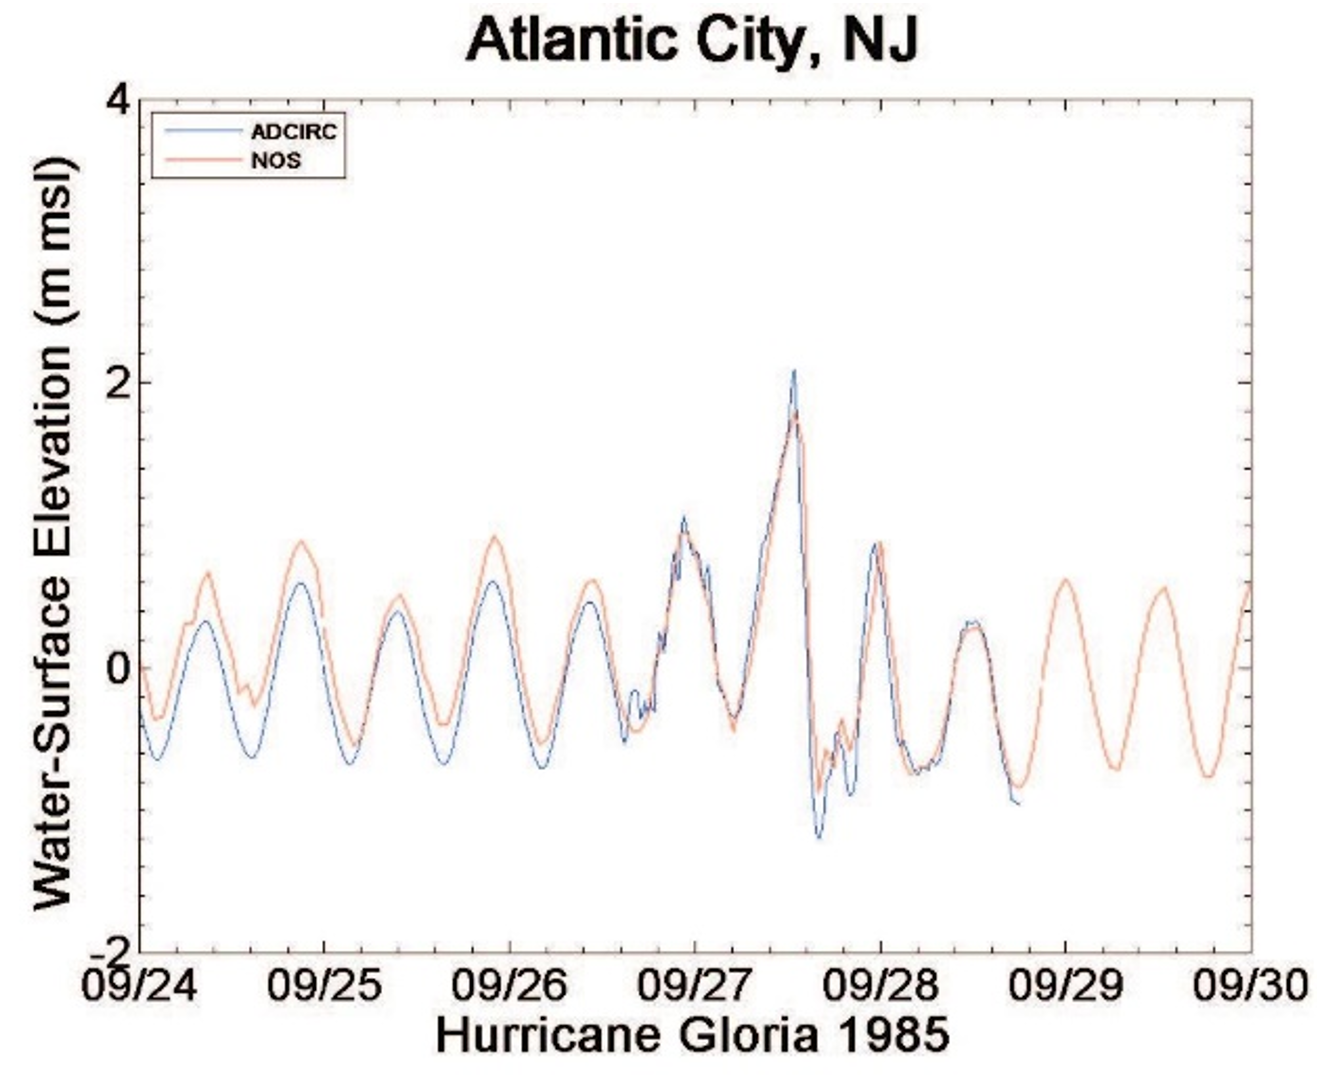
\includegraphics[width=0.5\textwidth, angle = 0]{Figures/surge_validation.png}
    \caption{Validation of surge simulation in Atlantic City using coupled ADCIRC-STWAVE for historical storm Hurricane Gloria, courtesy of USACE (Nadal-Carabbalo et al., 2015)}
    \label{fig:surge_validation}
\end{figure}

\subsection{Wave run up overland}

Even when coupled with an appropriate nearshore wave model, surge models simulate only the storm-surge elevation and not the additional impact of wave run up, which is particularly important for predicting losses to buildings and infrastructure in a storm event. Supplementary wave run-up simulations are required to capture the interaction of the waves with the shoreline and any coastal protective features along coastal transects. Two types of models are common:

\begin{enumerate}
    \item Wave-Group Envelope models, where the effects of unsteady wave groups on long-wave surge and runup drive time-varying water levels in the nearshore and at the moving shoreline. However, these models do not model individual wave runup, which can be important in certain instances. By far the most common model of this type is XBeach (Roelvink et al., 2009), which is also commonly used to estimate morphological evolution over short time periods. Models of this type require O(10m) resolution to resolve important processes, and thus have much heavier computational requirements than both spectral wave and surge models for a similar domain. Thus, they are generally limited to km-to-tens of km-scales for simulations. 
    \item Wave-resolving models, where individual points on the water surface are defined to model the evolution of the detailed wave shape over arbitrary bathymetry. The most common models of this type use different versions of Boussinesq models (Lynett et al., 2002; Kennedy et al., 2000; Nwogu and Demirbilek, 2010), which are derived from Taylor series expansions about the long wave limit. Wave-resolving models can simulate both wave group runup and runup from individual waves, but may require resolution of O(5m) or finer in the nearshore. Although these models may be used to simulate nearshore behavior of entire storms, they are quite computationally expensive (far more so than wave-group envelope models), and often one-dimensional transects are chosen for representative simulations. Transect locations are generally selected by segmenting the defined coastline in the areas of interest and selecting the transect density proportional to computational demand. Each transect is then discretized to capture the site-specific bathymetry (offshore) and topography (onshore) along its length. Moreover, transects must accurately capture the current condition of coastal protective features, e.g., dunes, in order to effectively predict the total run up inland. Inputs from the surge and spectral wave models are fed into a one-dimensional (1D) Boussinesq model executed at the pre-selected transects in order to estimate the wave run up overland (Demirbilek et al., 2009). 
\end{enumerate}

\subsection{Surrogate modeling approach}

Given the high degree of sophistication and computational resources required to execute just one high-fidelity simulation (e.g., an ADCIRC+STWAVE/SWAN run), alternative simulation tools have been developed recently to enable a wider range of users to employ these models for hazard characterization, risk assessment, and design of coastal protective strategies. Most notably, surrogate modeling approaches can efficiently evaluate hurricane wave and surge responses by leveraging databases of existing high-fidelity simulations normally driven by a collection of historical and synthetic hurricane tracks (USACE, 2015). This is made possible by formulating a simplified description of a storm scenario by a small number of model parameters corresponding to its characteristics at landfall. The scenarios in the database are then parameterized with respect to this model parameter vector and ultimately provide an input–output dataset. Because the geospatial representation often covers a regional coastline (typically represented by a large number of nodes) and resolves the coastal hazards at different times during the hurricane’s history, the dataset is often high-dimensional. After correcting for any dry nodes at inland locations, the surrogate model is then built to approximate this input-output relationship. 

Although the initial implementations of the surrogate modeling approach relied upon a moving least-squares-response surface methodology, more recent implementations for natural hazard risk assessment now employ a Kriging metamodel for this purpose (Jia and Taflanidis, 2013). To further reduce the computational burden pertaining to both speed of execution and more importantly memory requirements, this approach is coupled with principal component analysis (PCA) as a dimensional reduction technique. The metamodel is then developed in this low-dimensional latent space (in this case below 100), with the predictions transformed back to the original space for visualization purposes. This PCA implementation contributes to very large computational savings necessary to enable the evaluation of a large ensemble of scenarios as required for a probabilistic evaluation while circumventing the need for HPC resources (Jia and Taflanidis, 2013). Validation of these surrogate models using leave-one-out cross validation (Taflanidis et al., 2017) suggested high accuracy, with coefficient of determination close to 0.96 and a correlation coefficient close to 98\%. By permitting rapid evaluation of alternate storm scenarios, surrogate models offer an effective way to communicate simulation results to urban planners and emergency managers. One such implementation is a software system developed to assess storm surge risks on the coast of New Jersey (NJcoast, 2018a).

\section{Required Inputs and Resulting Outputs}
\label{sec:storm_surge_io}

High-fidelity computational simulations of coastal hazards require: (1) storm track information, including the relevant description of the hurricane wind and pressure fields to drive the model; (2) the topography and bathymetry along the coastline; and (3) the land use/land cover data for the simulation of wave run up on shore. The simulations are inherently sensitive to assumptions made regarding tides at the time of landfall. The coupling of a storm surge + nearshore wave + wave run-up model will yield geospatially-distributed, time-dependent responses, i.e., the mean water elevation, max water elevation, max water depth, and significant wave height (or limit of moderate wave action). Such responses can be generated either by the coupling of the aforementioned high-fidelity models or a surrogate model tuned to a database of results from these models. A brief summary of specific inputs required for storm surge models, the wave run-up models, and the related surrogate models are as follows:
\newline

\noindent\textbf{Storm Surge Models} \\All storm surge models require variations of the same inputs, potentially in much different forms. All models require:

\begin{itemize}
    \item Spatial and temporal information about wind fields and pressure. This may be in the form of gridded data, or in the form of parameterized wind and pressure fields,
    \item Bathymetry and topography over the entire domain,
    \item Frictional information, whether in the form of direct frictional coefficients or roughness, or land use/land cover information that is converted to frictional resistance. 
    \item Boundary conditions at the domain limits
\end{itemize}

\noindent
Many models will also require:

\begin{itemize}
    \item Information on tidal forcing when real dates are being simulated
    \item Computational settings, particularly for parallel systems
\end{itemize}

\noindent\textbf{Wave Run-up Models} \\In addition to the topography and bathymetry data at each identified transect, and potentially frictional information, the wave run-up model must receive wave and water level inputs from the coupled wave-storm surge model.
\newline

\noindent\textbf{Surrogate Models} \\Inputs to the surrogate model are twofold: the primary input required to develop the surrogate model itself is the aforementioned database of high-fidelity simulations for a family of storm tracks that may include tropical and extra-tropical storms. Once developed, users of the surrogate model input only a collection of parameters necessary to describe the storm scenario based on its characteristics at landfall: 

\begin{enumerate}
    \item reference location (latitude, longitude)
    \item track heading (angle)
    \item central pressure (or pressure difference)
    \item forward speed
    \item radius of maximum winds
\end{enumerate}

More recently, this implementation was further simplified to enable simulation based on only reference location and storm strength (Category 1-5) (NJcoast, 2018a). It is important to emphasize that once the surrogate model is tuned to high-fidelity simulation data for a specific geographic location, it can efficiently provide predictions for storm scenarios of varying characteristics, even if that scenario does not match any of those within the original database of high-fidelity simulations. 

\section{Primary Software Environments}
\label{sec:storm_surge_tools}

The execution environments are briefly summarized below, but only for models included in the NHERI DesignSafe suite. 
\newline

\noindent\textbf{ADCIRC and coupled models} \\ADCIRC has been optimized by unrolling loops for enhanced performance on multiple computer architectures and can be executed on any operating system with a working FORTRAN compiler. These include large commercial Unix systems (IBM Power & Blue Gene, Cray, SGI, and Sun), Linux- and FreeBSD-based clusters, and personal workstations running Windows or Mac OSX. ADCIRC includes MPI library calls to allow it to operate at high efficiency on parallel computer architectures, which is often preferable for simulations over large domains where a single hurricane realization can require thousands of CPU hours. Coupled ADCIRC+SWAN models are available on all of the aforementioned platforms (with the exception of Windows), while the coupled ADCIRC+STWAVE model is available on all the platforms including Windows PCs as part of the Coastal Storm Modeling System (CSTORM-MS). ADCIRC and its parallel implementation, PADCIRC, along with the coupled ADCIRC+SWAN software, are available on DesignSafe.
\newline

\noindent\textbf{CLAWPACK/GEOCLAW} \\Clawpack (“Conservation Laws Package”) is a collection of finite-volume methods for linear and nonlinear hyperbolic systems of conservation laws. Clawpack employs high-resolution Godunov-type methods with limiters in a general framework applicable to many kinds of waves. GEOCLAW is an open-source, finite-volume, wave-propagation software, which is implemented in CLAWPACK, to estimate hurricane-induced storm surge with adaptive mesh refinement. The CLAWPACK 5.4.0 suite and the GEOCLAW tools are available through DesignSafe.
\newline

\noindent\textbf{SLOSH} \\SLOSH (Sea, Lake and Overland Surges from Hurricanes) is a computerized numerical model developed by the National Weather Service (NWS) to estimate storm-surge heights determined from historical, hypothetical, or predicted hurricanes by taking into account the atmospheric pressure, size, forward speed, and track data. These parameters are used to create a model of the wind field that drives the storm surge. The SLOSH model consists of a set of physics equations that are applied to a specific locale's shoreline to incorporate the unique bay and river configurations, water depths, bridges, roads, levees, and other physical features. Storm-surge forecasts developed using SLOSH are available at https://www.nhc.noaa.gov/surge/slosh.php.

\section{Major Research Gaps}
\label{sec:storm_surge_gaps}

Although many research topics remain, the major issue remaining with storm surge models is that the fast models are less accurate, and the accurate models are slow. Thus, it remains impossible to run the most accurate models for the hundreds or thousands of simulations required to obtain surge probabilities prior to a landfalling hurricane, or to simulate very long climatological records. Three methodologies hold the potential to improve the accuracy/speed tradeoff:

\begin{itemize}
    \item Surrogate or reduced models that make use of previous high fidelity model runs to develop simpler and faster models for new cases. This was discussed earlier; AI also falls into this broad category,
    \item Improved computational schemes that improve parallel performance for slower models, or improve accuracy for faster models,
    \item Improved theoretical schemes to increase the accuracy on coarse grids. The subgrid model corrections fall into this category, and have been shown to increase accuracy greatly (Kennedy et al., 2019).
\end{itemize}

The next major research gap is very difficult but extremely important: large scale surge models do not account for morphological evolution during storms. Dune or beach erosion, and levee failure, are two examples of morphological feedbacks that may affect significantly surge inundation, and estimates of post-storm erosion are also greatly desired. This has been a long-term goal with little progress.

Finally, whether employing these high-fidelity models or a companion surrogate model, the resulting time-evolving water depth and velocity must translate into loadings on buildings and infrastructure. In this regard, these models face similar limitations as wind-field models given the complexity of interactions with their surroundings. Accurately capturing the physics of the flow overland and the effect of its interaction with the built environment on the load description remains a challenging problem, even without further accounting for the effects of debris transported in the flow. Identifying means to reasonably determine the impact of these interactions on the load description—without having to support an intensive CFD investigation—will enable a wider range of researchers to evaluate the impacts of coastal hazards. 
 
\section{References}

% TODO: These references shall be moved to the references.bib file.

% Chen, C.S., Liu, H.D., Beardsley, R.C. (2003). An unstructured grid, finite-volume, three-dimensional, primitive equations ocean model: Application to coastal ocean and estuaries. Journal of Atmospheric and Oceanic Technology. 20(1), 159-186.

% Dietrich, J.C., Zijlema, M., Westerink, J.J., Holthuijsen, L.H., Dawson, C., Luettich, R.A., Jensen, R.E., Smith, J.M., Stelling, G.S., and Stone, G.W. (2011). Modeling hurricane waves and storm surge using integrally-coupled, scalable computations. Coastal Engineering 58, 45-65. 

% Hu, K., Chen, Q., Wang, H. (2015). A numerical study of vegetation impact on reducing storm surge by wetlands in a semi-enclosed estuary. Coastal Engineering 95, 66-76.

% Lynett, P.J., Wu, T.R., Liu, P.L.-F. (2002). Modeling wave runup with depth-integrated equations. Coastal Engineering 46(2), 89-107.

% Kennedy, A.B., Chen, Q., Kirby, J.T., and Dalrymple, R.A. (2000). Boussinesq modeling of wave transformation, breaking and runup. I: 1D. J. Waterway, Port, Coastal and Ocean Eng.-ASCE, 126, 39-47.

% Kennedy, A.B., Wirasaet, D., Begmohammadi, A., Sherman, T., Bolster, D., and Dietrich, J.C. (2019). Subgrid theory for storm surge modeling. Ocean Modelling 144, 101491, doi: 10.1016/j.ocemod.2019.101491.

% Kerr, P.C., Donahue, A.S., Westerink, J.J., Luettich, R.A., Zheng, L.Y., Weisberg, R.H., Huang, Y., Wang, H.V., Teng, Y., Forrest, D., Zhang, Y.J., Roland, A., Haase, A.T., Kramer, A., Taylor, A., Rhome, J.R., Feyen, J., Signell, R.P., Hanson, J., Hope, M.E., Estes, R., Dominguez, R., Dunbar, R., Semeraro, L., Westerink, H.J., Kennedy, A., Smith, J.M., Powell, M.D., Cardone, V.J., and Cox, A.T. (2013). U.S. IOOS Coastal & Ocean Modeling Testbed: Inter-Model Evaluation of Tides, Waves, and Hurricane Surge in the Gulf of Mexico, J. Geophys. Res.-Oceans, 118, 5129-5172, doi: 10.1002/jgrc.20376.

% Nwogu, O., and Demirbilek, Z. (2010). Infragravity Wave Motions and Runup over Shallow Fringing Reefs. J. Waterway, Port, Coastal and Ocean Eng.-ASCE, 136, 295-305. 

% Rego, J.L., Li, C.Y., (2010). Storm surge propagation in Galveston Bay during Hurricane Ike. Journal of Marine Systems. 82(4), 265-279.

% Roelvink, D., Reniers, A., van Dongeren, A., de Vries, J.V., McCall, R., and Lescinski, J. (2009). Modelling storm impacts on beaches, dunes, and barrier islands. Coastal Engineering 56(11-12), 1133-1152.

% Smith, J.M., Hesser, T., Roland, A., and Bryant, M. (2018). Validation of unstructured Wavewatch III for nearshore waves. In: P. Lynett, Ed. Proc. 36th Conf. Coastal Eng., Baltimore, ASCE, https://journals.tdl.org/icce/index.php/icce/article/view/8324 

% Vousdoukas, M.I., Voukouvalas, E., Annunziato, A., Giardino, A., Feyen, L. (2016). Projections of extreme storm surge levels along Europe. Climate Dynamics 47(9), 3171-3190.

% Zhang, K/. Li, Y., and Zachry, B. (2017). Transition of the Coastal and Estuarine Storm Tide Model to an Operational Model for Forecasting Storm Surges. In: Abstracts, 33rd Conference on Hurricanes and Tropical Meteorology, Ponte Vedra, Paper7B.4, https://ams.confex.com/ams/33HURRICANE/webprogram/Paper340466.html 

% Zijlema, M. (2010). Computation of wind-wave spectra in coastal waters with SWAN on unstructured grids. Coastal Engineering 57, 267-277.

% TODO: Not all of the references below belong to this chapter

% Anastasopoulos, I., and Gazetas, G. (2007). Foundation–structure systems over a rupturing normal fault: Part II. Analysis of the Kocaeli case histories. Bulletin of Earthquake Engineering 5, 277–301.

% Anastasopoulos, I., Callerio, A., Bransby, M., Davies, M., El Nahas, A., Faccioli, E., Gazetas, G., Masella, A., Paolucci, R., Pecker, A., et al. (2008). Numerical analyses of fault–foundation interaction. Bulletin of Earthquake Engineering 6, 645–675.

% ADCIRC: https://adcirc.org/

% T. D. Ancheta, R. B. Darragh, J. P. Stewart, E. Seyhan, W. J. Silva, B. S.-J. Chiou, K. E. Wooddell, R. W. Graves, A. R. Kottke, D. M. Boore, T. Kishida and J. L. Donahue, "NGA-West2 Database," Earthquake Spectra, vol. 30, no. 3, pp. 989-1005, 2014.

% Andrus, R.D., and Stokoe II, K.H. (2000). Liquefaction resistance of soils from shear-wave velocity. Journal of Geotechnical and Geoenvironmental Engineering 126, 1015–1025.

% Barbato, M., Petrini, F., Unnikrishnan, V. U., and Ciampoli, M. (2013). "Performance-Based Hurricane Engineering (PBHE) framework." Structural Safety, 45, 24-35.

% Berrill, J. (1983). Two-dimensional analysis of the effect of fault rupture on buildings with shallow foundations. International Journal of Soil Dynamics and Earthquake Engineering 2, 156–160.

% Bommer J.J., Scherbaum F. (2008) The Use and misuse of Logic Trees in Probabilistic Seismic Hazard Analysis, Earthquake Spectra, 24:997-1009

% Boulanger, R., and Ziotopoulou, K. (2015). PM4Sand (Version 3): A sand plasticity model for earthquake engineering applications. Center for Geotechnical Modeling Report No. UCD/CGM-15/01, Department of Civil and Environmental Engineering, University of California, Davis, Calif.

% Bransby, M., Davies, M., and Nahas, A.E. (2008a). Centrifuge modelling of normal fault–foundation interaction. Bulletin of Earthquake Engineering 6, 585–605.

% Bransby, M., Davies, M., El Nahas, A., and Nagaoka, S. (2008b). Centrifuge modelling of reverse fault–foundation interaction. Bulletin of Earthquake Engineering 6, 607–628.

% Bray, J.D. (2001). Developing mitigation measures for the hazards associated with earthquake surface fault rupture. In Workshop on Seismic Fault-Induced Failures—Possible Remedies for Damage to Urban Facilities. University of Tokyo Press, pp. 55–79.

% Bray, J.D., Boulanger, R.W., Cubrinovski, M., Tokimatsu, K., Kramer, S.L., O’Rourke, T., Rathje, E., Green, R.A., Robertson, P.K., and Beyzaei, C.Z. (2017). U.S. – New Zealand – Japan International Workshop on “Liquefaction-Induced Ground Movements Effects (University of California, Berkeley: Pacific Earthquake Engineering Research Center).

% Bray, J.D., and Travasarou, T. (2007). Simplified procedure for estimating earthquake-induced deviatoric slope displacements. Journal of Geotechnical and Geoenvironmental Engineering 133, 381–392.

% Bray, J.D., and Travasarou, T. (2009). Pseudostatic coefficient for use in simplified seismic slope stability evaluation. Journal of Geotechnical and Geoenvironmental Engineering 135, 1336–1340.

% Bray, J.D., Macedo, J., and Travasarou, T. (2017). Simplified Procedure for Estimating Seismic Slope Displacements for Subduction Zone Earthquakes. Journal of Geotechnical and Geoenvironmental Engineering 144, 04017124.

% Byrne, P.M., Park, S.-S., Beaty, M., Sharp, M., Gonzalez, L., and Abdoun, T. (2004). Numerical modeling of liquefaction and comparison with centrifuge tests. Canadian Geotechnical Journal 41, 193–211.

% Cetin, K.O., and Seed, R.B. (2004). Nonlinear shear mass participation factor (rd) for cyclic shear stress ratio evaluation. Soil Dynamics and Earthquake Engineering 24, 103–113.

% Chavas, D. R., and Lin, N. (2016). "A Model for the Complete Radial Structure of the Tropical Cyclone Wind Field. Part II: Wind Field Variability." Journal of the Atmospheric Sciences, 73(8), 3093-3113.

% Chavas, D. R., Lin, N., and Emanuel, K. (2015). "A Model for the Complete Radial Structure of the Tropical Cyclone Wind Field. Part I: Comparison with Observed Structure." Journal of the Atmospheric Sciences, 72(9), 3647-3662.

% Chen, Y., and Duan, Z. (2018). "A statistical dynamics track model of tropical cyclones for assessing typhoon wind hazard in the coast of southeast China." Journal of Wind Engineering and Industrial Aerodynamics, 172, 325-340.

% Chow, S.-h. (1971). A Study of the Wind Field in the Planetary Boundary Layer of a Moving Tropical Cyclone. Master of Science, New York University, New York, N.Y.

% Chuang, W.-C., and Spence, S. M. J. (2019). "An efficient framework for the inelastic performance assessment of structural systems subject to stochastic wind loads." Engineering Structures, 179, 92-105.

% Cole Jr, D.A., and Lade, P.V. (1984). Influence zones in alluvium over dip-slip faults. Journal of Geotechnical Engineering 110, 599–615.

% C. Crouse, J. T. H., K. R. Milner, C. A. Goulet, S. Callaghan and R. W. Graves, "Site-Specific MCER Response Spectra for Los Angeles Region based on 3-D Numerical Simulations and the NGA West2 Equations," in 11th National Conference in Earthquake Engineering, Los Angeles, 2018.

% Cornell, C.A. (1968). Engineering seismic risk analysis, Bull. Seism. Soc. Am., 58, 1583-1606

% Cornell C.A., Bazzurro P. (1999) Disaggregation of seismic hazard, Bull. Seism. Soc. Am., 89:501-520

% Cubrinovski, M., Bradley, B., Wotherspoon, L., Green, R., Bray, J., Wood, C., Pender, M., Allen, J., Bradshaw, A., Rix, G., et al. (2011). Geotechnical Aspects of the 22 February 2011 Christchurch Earthquake.

% Cubrinovski, M., Bray, J., de la Torre, C., Olsen, 497 M, Bradley, B., Chiaro, G., Stock, E., and Wotherspoon, L. (2017). Liquefaction Effects and Associated Damages Observed at the Wellington CentrePort from the 2016 Kaikoura Earthquake.

% Danciu, L., Şeşetyan, K., Demircioglu, M. et al. (2017) The 2014 Earthquake Model of the Middle East: seismogenic sources, Bull Earthquake Eng (2018) 16: 3465. 

% Davis, C., Wang, W., Chen, S. S., Chen, Y., Corbosiero, K., DeMaria, M., Dudhia, J., Holland, G., Klemp, J., Michalakes, J., Reeves, H., Rotunno, R., Snyder, C., and Xiao, Q. (2008). "Prediction of Landfalling Hurricanes with the Advanced Hurricane WRF Model." Monthly Weather Review, 136(6), 1990-2005.

% Demirbilek, Z., O.G. Nwogu, D.L Ward and A. Sanchez, A. (2009) "Wave transformation over reefs: evaluation of one dimensional numerical models." Report ERDC/CHL TR-09-1, US Army Corps of Engineers.

% Douglas J. (2018) Ground Motion Prediction Equations 1964-2018, Dept. of Civil and Env. Engineering, University of Strathclyde, Glasgow, UK

% Y. Cui, K. B. Olsen, T. H. Jordan, K. Lee, J. Zhou, P. Small, D. Roten, G. Ely, D. K. Panda, A. Chourasia, J. Levesque, S. M. Day and P. Maechling, "Scalable Earthquake Simulation on Petascale Supercomputers," in Proceedings of the 2010 ACM/IEEE International Conference for High Performance Computing, Networking, Storage and Analysis, New Orleans, LA, 2010.

% Emanuel, K. (2004). "Tropical cyclone energetics and structure." Atmospheric Turbulence and Mesoscale Meteorology: Scientific Research Inspired by Doug Lilly, B. Stevens, E. Fedorovich, and R. Rotunno, eds., Cambridge University Press, Cambridge, 165-192.

% Emanuel, K. (2005). "Increasing destructiveness of tropical cyclones over the past 30 years." Nature, 436(7051), 686-688.

% Emanuel, K. (2011). "Self-Stratification of Tropical Cyclone Outflow. Part II: Implications for Storm Intensification." Journal of the Atmospheric Sciences, 69(3), 988-996.

% Emanuel, K. (2017). "A fast intensity simulator for tropical cyclone risk analysis." Natural Hazards, 88(2), 779-796.

% Emanuel, K., DesAutels, C., Holloway, C., and Korty, R. (2004). "Environmental Control of Tropical Cyclone Intensity." Journal of the Atmospheric Sciences, 61(7), 843-858.

% Emanuel, K., Ravela, S., Vivant, E., and Risi, C. (2006). "A Statistical Deterministic Approach to Hurricane Risk Assessment." Bull. Amer. Meteorol. Soc., 87(3), 299-314.

% Emanuel, K., and Rotunno, R. (2011). "Self-Stratification of Tropical Cyclone Outflow. Part I: Implications for Storm Structure." Journal of the Atmospheric Sciences, 68(10), 2236-2249.

% Emanuel, K., Sundararajan, R., and Williams, J. (2008). "Hurricanes and Global Warming: Results from Downscaling IPCC AR4 Simulations." Bull. Amer. Meteorol. Soc., 89(3), 347-368.

% Emanuel, K. A. (1988). "The Maximum Intensity of Hurricanes." Journal of the Atmospheric Sciences, 45(7), 1143-1155.

% ESDU (1983) Strong winds in the atmospheric boundary layer, part 2: discrete gust speeds, Engineering Sciences Data Unit Item No. 83045, London, England.

% Fang, G., Zhao, L., Cao, S., Ge, Y., and Pang, W. (2018a). "A novel analytical model for wind field simulation under typhoon boundary layer considering multi-field correlation and height-dependency." Journal of Wind Engineering and Industrial Aerodynamics, 175, 77-89.

% Fang, G., Zhao, L., Song, L., Liang, X., Zhu, L., Cao, S., and Ge, Y. (2018b). "Reconstruction of radial parametric pressure field near ground surface of landing typhoons in Northwest Pacific Ocean." Journal of Wind Engineering and Industrial Aerodynamics, 183, 223-234.

% E. H. Field, R. J. Arrowsmith, G. P. Biasi, P. Bird, T. E. Dawson, K. R. Felzer, D. D. Jackson, K. M. Johnson, T. H. Jordan, C. Madden, A. J. Michael, K. R. Milner, M. T. Page, T. Parsons and P. M. Powers, "Uniform California Earthquake Rupture Forecast, Version 3 (UCERF3)—The Time‐Independent Model," Bulletin of the Seismological Society of America, vol. 104, no. 3, pp. 1122-1180, 2014.

% E. H. Field, T. H. Jordan and C. A. Cornell, "OpenSHA: A Developing Community-Modeling Environment for Seismic Hazard Analysis," Seismological Research Letters, vol. 74, no. 74, pp. 406-419, 2003.

% Garcia, F.E., and Bray, J.D. (2018a). Distinct Element Simulations of Shear Rupture in Dilatant Granular Media. International Journal of Geomechanics 18, 04018111.

% Garcia, F.E., and Bray, J.D. (2018b). Distinct element simulations of earthquake fault rupture through materials of varying density. Soils and Foundations 58, 986–1000.

% Garcia J., Pagani M., Rodriguez L., Weatherill G. (2018) Creation of a new PSHA input model for South America and calculation of results, GEM SARA Wiki, Available at https://sara.openquake.org/hazard_rt7 (Accessed: 21 Nov. 2018)

% Georgiou, P. N. (1986). Design Wind Speeds In Tropical Cyclone-prone Regions. Ph. D., University of Western Ontario.

% Giardini, D., Woessner J. , Danciu L. (2014) Mapping Europe’s Seismic Hazard. EOS, 95(29): 261-262.

% Goulet C.A., Bozorgnia Y., Kuehn N., Atik L.A., Youngs R.R., Graves R.W., Atkinson G.M. (2017) NGA-East Ground-Motion Models for the U.S. Geological Survey National Seismic Hazard Maps, PEER Report No. 2017/03, Pacific Earthquake Engineering Research Center, UC Berkeley, California, US

% Hamid, S., Golam Kibria, B. M., Gulati, S., Powell, M., Annane, B., Cocke, S., Pinelli, J.-P., Gurley, K., and Chen, S.-C. (2010). "Predicting losses of residential structures in the state of Florida by the public hurricane loss evaluation model." Statistical Methodology, 7(5), 552-573.

% Holland, G. (2008). "A Revised Hurricane Pressure–Wind Model." Monthly Weather Review, 136(9), 3432-3445.

% Holland, G. J. (1980). "An Analytic Model of the Wind and Pressure Profiles in Hurricanes." Monthly Weather Review, 108(8), 1212-1218.

% Holland, G. J., Belanger, J. I., and Fritz, A. (2010). "A Revised Model for Radial Profiles of Hurricane Winds." Monthly Weather Review, 138(12), 4393-4401.

% Hu, L., Xu, Y.-L., Zhu, Q., Guo, A., and Kareem, A. (2017). "Tropical Storm–Induced Buffeting Response of Long-Span Bridges: Enhanced Nonstationary Buffeting Force Model." Journal of Structural Engineering, 143(6), 04017027.

% Huang, W. F., and Xu, Y. L. (2013). "Prediction of typhoon design wind speed and profile over complex terrain." Struct. Eng. Mech., 45(1), 1-18.

% Hynes-Griffin, M.E., and Franklin, A.G. (1984). Rationalizing the Seismic Coefficient Method. (Army Engineer Waterways Experiment Station Vicksburg Ms Geotechnical Lab).

% Idriss, I. (1999). An update to the Seed-Idriss simplified procedure for evaluating liquefaction potential. Proc., TRB Worshop on New Approaches to Liquefaction, FHWA-RD-99-165, Federal Highway Administration.

% Idriss, I., and Boulanger, R. (2014). CPT and SPT based Liquefaction Triggering Procedures. Centre for Geotechnical Modelling.

% Idriss, I.M., and Boulanger, R.W. (2008). Soil Liquefaction during Earthquakes (Earthquake Engineering Research Institute).

% Ishihara, T., Siang, K. K., Leong, C. C., and Fujino, Y. (2005). "Wind Field Model and Mixed Probability Distribution Function for Typhoon Simulation " The Sixth Asia-Pacific Conference on Wind Engineering (APCWE-VI)Seoul, Korea.

% Jacob, K., Deodatis, G., Atlas, J., Whitcomb, M., Lopeman, M., Markogiannaki, O., Kennett, Z., Morla, A., Leichenko, R. and Vancura, P. (2011). “Responding to Climate Change in New York State: The ClimAID Integrated Assessment for Effective Climate Change Adaptation in New York State: Transportation,” Annals of the New York Academy of Sciences, Vol. 1244, No. 1, pp. 299-362.

% Jia G. and A. A. Taflanidis (2013) "Kriging metamodeling for approximation of high-dimensional wave and surge responses in real-time storm/hurricane risk assessment," Computer Methods in Applied Mechanics and Engineering, vol. 261-262, pp. 24-38.

% Jia G., A. A. Taflanidis, N. C. Nadal-Caraballo, J. Melby, A. Kennedy, and J. Smith (2015) "Surrogate modeling for peak and time dependent storm surge prediction over an extended coastal region using an existing database of synthetic storms," Natural Hazards, vol. 81, pp. 909-938.

% Jibson, R.W. (2007). Regression models for estimating coseismic landslide displacement. Engineering Geology 91, 209–218.

% Kareem, A., Hu, L., Guo, Y., and Kwon, D. K. (2018). "Generalized wind loading chain: A time-frequency modeling framework for nonstationary winds effects on structures." Journal of Structural Engineering, ASCE, Submitted.

% Kavazanjian, E., Andrade, J., Arulmoli, K.A., Atwater, B.F., Christian, J.T., Green, R., Kramer, S.L., Mejia, L., Mitchell, J.K., Rathje, E., et al. (2016). State of the Art and Practice in the Assessment of Earthquake-Induced Soil Liquefaction and Its Consequences (Washington, DC: The National Academies Press).

% Kayen, R., Moss, R., Thompson, E., Seed, R., Cetin, K., Kiureghian, A.D., Tanaka, Y., and Tokimatsu, K. (2013). Shear-wave velocity–based probabilistic and deterministic assessment of seismic soil liquefaction potential. Journal of Geotechnical and Geoenvironmental Engineering 139, 407–419.

% Kennedy, A.B., Gravois, U., Zachry, B.C., Westerink, J.J., Hope, M.E., Dietrich, J.C., Powell, M.D., Cox, A.T., Luettich, R.L., Dean, R.G. (2011) "Origin of the Hurricane Ike forerunner surge," Geophysical Research Letters L08805. 

% Kennedy, A.B., Westerink, J.J., Smith, J., Taflanidis, A.A., Hope, M., Hartman, M., Tanaka, S., Westerink, H., Cheung, K.F., Smith, T., Hamman, M., Minamide, M., Ota, A. (2012) "Tropical cyclone inundation potential on the Hawaiian islands of Oahu and Kauai," Ocean Modelling. 52-53, 54-68. 

% Kepert, J. (2001). "The Dynamics of Boundary Layer Jets within the Tropical Cyclone Core. Part I: Linear Theory." Journal of the Atmospheric Sciences, 58(17), 2469-2484.

% Kepert, J., and Wang, Y. (2001). "The Dynamics of Boundary Layer Jets within the Tropical Cyclone Core. Part II: Nonlinear Enhancement." Journal of the Atmospheric Sciences, 58(17), 2485-2501.

% Kepert, J. D. (2006). "Observed Boundary Layer Wind Structure and Balance in the Hurricane Core. Part II: Hurricane Mitch." Journal of the Atmospheric Sciences, 63(9), 2194-2211.

% Kepert, J. D. (2010a). "Slab‐ and height‐resolving models of the tropical cyclone boundary layer. Part I: Comparing the simulations." Quarterly Journal of the Royal Meteorological Society, 136(652), 1686-1699.

% Kepert, J. D. (2010b). "Slab‐ and height‐resolving models of the tropical cyclone boundary layer. Part II: Why the simulations differ." Quarterly Journal of the Royal Meteorological Society, 136(652), 1700-1711.

% Kepert, J. D. (2011). "Choosing a Boundary Layer Parameterization for Tropical Cyclone Modeling." Monthly Weather Review, 140(5), 1427-1445.

% Kepert, J. D. (2013). "How Does the Boundary Layer Contribute to Eyewall Replacement Cycles in Axisymmetric Tropical Cyclones?" Journal of the Atmospheric Sciences, 70(9), 2808-2830.

% Kepert, J. D., and Nolan, D. S. (2014). "Reply to “Comments on ‘How Does the Boundary Layer Contribute to Eyewall Replacement Cycles in Axisymmetric Tropical Cyclones?’”." Journal of the Atmospheric Sciences, 71(12), 4692-4704.

% Kijewski-Correa, T., Smith, N., Taflanidis, A., Kennedy, A., Liu, C., Krusche, M., and Vardeman, C., "CyberEye: Development of integrated cyber-infrastructure to support rapid hurricane risk assessment," Journal of Wind Engineering and Industrial Aerodynamics, vol. 133, pp. 211-224, 2014.

% Kwon, D.-K., and Kareem, A. (2009). "Gust-Front Factor: A New Framework for Wind Load Effects on Structures." Journal of Structural Engineering, ASCE.

% Langousis, A. (2008). Extreme Rainfall Intensities and Long-term Rainfall Risk from Tropical Cyclones. Ph. D., Massachusetts Institute of Technology.

% Lauren, M., Yue, W., Chris, L., and David, R. (2014). "Assessing Climate Change Impact on the U.S. East Coast Hurricane Hazard: Temperature, Frequency, and Track." Natural Hazards Review, 15(3).

% LeVeque, R. (2002). Finite Volume Methods for Hyperbolic Problems, Cambridge Texts in Applied Mathematics, Cambridge University Press.

% Li, L., Kareem, A., Hunt, J., Xiao, Y., Zhou, C., and Song, L. (2015a). "Turbulence Spectra for Boundary-Layer Winds in Tropical Cyclones: A Conceptual Framework and Field Measurements at Coastlines." Boundary-Layer Meteorol, 154(2), 243-263.

% Li, L., Kareem, A., Xiao, Y., Song, L., and Zhou, C. (2015b). "A comparative study of field measurements of the turbulence characteristics of typhoon and hurricane winds." Journal of Wind Engineering and Industrial Aerodynamics, 140, 49-66.

% Li, S. H., Duan, Z. D., and Hong, H. P. (2016). "Typhoon Wind Hazard Estimation and Mapping for Coastal Region in Mainland China." Natural Hazards Review, 17(2).

% Li, S. H., and Hong, H. P. (2015). "Observations on a Hurricane Wind Hazard Model Used to Map Extreme Hurricane Wind Speed." Journal of Structural Engineering, 141(10), 04014238.

% Li, S. H., and Hong, H. P. (2016). "Typhoon wind hazard estimation for China using an empirical track model." Natural Hazards, 82(2), 1009-1029.

% Lin, J.-S., and Whitman, R.V. (1986). Earthquake induced displacements of sliding blocks. Journal of Geotechnical Engineering 112, 44–59.

% Lin, N. (2015). "An Integrated Approach to Assess and Manage Hurricane Risk in a Changing Climate." The Bridge, 45(4), 46-51.

% Lin, N., and Chavas, D. (2012). "On hurricane parametric wind and applications in storm surge modeling." Journal of Geophysical Research: Atmospheres, 117(D9).

% Liu, F. (2014). Projections of Future US Design Wind Speeds cue to Climate Change for Estimating Hurricane Losses. Ph.D., Clemson University.

% Liu, Y., Zhang, D.-L., and Yau, M. K. (1997). "A Multiscale Numerical Study of Hurricane Andrew (1992). Part I: Explicit Simulation and Verification." Monthly Weather Review, 125(12), 3073-3093.

% Luettich R.A, J. J. Westerink, and N. W. Scheffner (1992), ADCIRC: An advanced three-dimensional circulation model for shelves, coasts, and estuaries. Report 1. Theory and methodology of ADCIRC-2DDI and ADCIRC-3DL, Dredging Research Program Technical Report DRP-92-6, U.S Army Engineers Waterways Experiment Station, Vicksburg, MS.

% Macedo, J., Bray, J., Abrahamson, N., and Travasarou, T. (2018). Performance-Based Probabilistic Seismic Slope Displacement Procedure. Earthquake Spectra 34, 673–695.

% Maechling P.J., Silva F., Callaghan S. and Jordan T.H., "SCEC Broadband Platform: System Architecture and Software Implementation," Seismological Research Letters, vol. 86, no. 1, 2015.

% Makdisi, F.I., and Seed, H.B. (1978). Simplified procedure for estimating dam and embankment earthquake-induced deformations. Journal of Geotechnical and Geoenvironmental Engineering 104.

% Mandli, K.T., Ahmadia, A.J., Berger, M., Calhoun, D., George, D.L., Hadjimichael, Y., Ketcheson, D.I., Lemoine, G.I., LeVeque, R.J. (2016). Clawpack: building an open source ecosystem for solving hyperbolic PDEs. J. Computer Science 2(3):e68.

% Masters, F. J., Vickery, P. J., Bacon, P., and Rappaport, E. N. (2010). "TOWARD OBJECTIVE, STANDARDIZED INTENSITY ESTIMATES FROM SURFACE WIND SPEED OBSERVATIONS." Bull. Amer. Meteorol. Soc., 91(12), 1665-1681.

% Meng, Y., Matsui, M., and Hibi, K. (1995). "An analytical model for simulation of the wind field in a typhoon boundary layer." Journal of Wind Engineering and Industrial Aerodynamics, 56(2), 291-310.

% Meng, Y., Matsui, M., and Hibi, K. (1997). "A numerical study of the wind field in a typhoon boundary layer." Journal of Wind Engineering and Industrial Aerodynamics, 67-68, 437-448.

% Montgomery, M. T., Abarca, S. F., Smith, R. K., Wu, C.-C., and Huang, Y.-H. (2014). "Comments on “How Does the Boundary Layer Contribute to Eyewall Replacement Cycles in Axisymmetric Tropical Cyclones?”." Journal of the Atmospheric Sciences, 71(12), 4682-4691.

% Moss, R.E.S., and Ross, Z.E. (2011). Probabilistic fault displacement hazard analysis for reverse faults. Bulletin of the Seismological Society of America 101, 1542–1553.

% Mudd, L., Vickery, P., and Sarathi, P. (2015). "Development of a New Synthetic Hurricane Model for Deriving MetOcean Design Criteria for the Gulf of Mexico." Offshore Technology Conference, Offshore Technology Conference, Houston, Texas, USA.

% Mudd, L., and Vickery P.J. (2015). "Advancements in Synthetic Hurricane Track Modeling in the Gulf of Mexico." 14th International Conference on Wind Engineering,Porto Alegre, Brazil.

% Mueller C.S., Boyd O.S., Petersen M.D., Moschetti M.P., Rezaeian S., Shumway A.M. (2015) Siesmic Hazard in the Eastern United States, Earthquake Spectra, 31:85-107

% Nadal‐Caraballo N.C, J. A. Melby, V. M. Gonzalez, and A. T. Cox (2015), North Atlantic Coast Comprehensive Study – Coastal Storm Hazards from Virginia to Maine, ERDC/CHL TR-15-5 U.S. Army Engineer Research and Development Center, Vicksburg, MS.

% NJcoast (2018a) Storm Hazard Projection Tool, https://njcoast.us/documents/170/download/ 

% NJcoast (2018b) Implementation Report, https://njcoast.us/documents/164/download/ 

% NOAA Reanalysis Data (2018) www.aoml.noaa.gov/hrd/data_sub/re_anal.html, (Accessed: 11/14/2018)

% Oettle, N.K., and Bray, J.D. (2016). Numerical Procedures for Simulating Earthquake Fault Rupture Propagation. International Journal of Geomechanics 17, 04016025.

% Oettle, N.K., Bray, J.D., and Dreger, D.S. (2015). Dynamic effects of surface fault rupture interaction with structures. Soil Dynamics and Earthquake Engineering 72, 37–47.

% OpenFOAM: https://www.openfoam.com/

% Ordaz M., Martinelli F., D’Amico V., Meletti C. (2013) CRISIS2008: A flexible tool to perform probabilistic seismic hazard assessment, Seismological Research Letters 84:495-504, doi: 10.1785/0220120067

% Petersson N. and Sjogreen B., "SW4, version 2.01 [software]," Computational Infrastructure of Geodynamics, 2017. [Online]. Available: https://doi.org/10.5281/zenodo.1063644.

% Petersen, M.D., Dawson, T.E., Chen, R., Cao, T., Wills, C.J., Schwartz, D.P., and Frankel, A.D. (2011). Fault displacement hazard for strike-slip faults. Bulletin of the Seismological Society of America 101, 805–825.

% Powell, M., Soukup, G., Cocke, S., Gulati, S., Morisseau-Leroy, N., Hamid, S., Dorst, N., and Axe, L. (2005). "State of Florida hurricane loss projection model: Atmospheric science component." Journal of Wind Engineering and Industrial Aerodynamics, 93(8), 651-674.

% Powell, M. D., Vickery, P. J., and Reinhold, T. A. (2003). "Reduced drag coefficient for high wind speeds in tropical cyclones." Nature, 422, 279.

% Rathje, E.M., and Antonakos, G. (2011). A unified model for predicting earthquake-induced sliding displacements of rigid and flexible slopes. Engineering Geology 122, 51–60.

% Rathje, E.M., and Bray, J.D. (2000). Nonlinear coupled seismic sliding analysis of earth structures. Journal of Geotechnical and Geoenvironmental Engineering 126, 1002–1014.

% Rathje, E.M., Wang, Y., Stafford, P.J., Antonakos, G., and Saygili, G. (2014). Probabilistic assessment of the seismic performance of earth slopes. Bulletin of Earthquake Engineering 12, 1071–1090.

% Resio, D. T. and Westerink, J. J., "Modeling of the physics of storm surges," Physics Today, vol. 61, pp. 33-38, 2008.

% Robertson, P.K., and Wride, C.E. (1998). Evaluating cyclic liquefaction potential using the cone penetration test. Canadian Geotechnical Journal 35, 442–459.

% Russell, L. R. (1969). Probability Distributions for Texas Gulf Coast Hurricane Effects of Engineering Interest. 6917449 Ph.D., Stanford University, Ann Arbor.

% Saygili, G., and Rathje, E.M. (2008). Empirical predictive models for earthquake-induced sliding displacements of slopes. Journal of Geotechnical and Geoenvironmental Engineering 134, 790–803.

% Seed, H.B. (1979). Considerations in the earthquake-resistant design of earth and rockfill dams. Geotechnique 29, 215–263.

% Seed, H.B., and Idriss, I.M. (1971). Simplified procedure for evaluating soil liquefaction potential. Journal of Soil Mechanics & Foundations Div.

% Shapiro, L. J. (1983). "The Asymmetric Boundary layer Flow Under a Translating Hurricane." Journal of the Atmospheric Sciences, 40(8), 1984-1998.

% SLOSH: https://www.nhc.noaa.gov/surge/slosh.php

% Smith J.M, A. R. Sherlock, and D. T. Resio (2001) "STWAVE: Steady-state spectral wave model user's manual for STWAVE, Version 3.0," DTIC Document.

% Smith, R. K. (1968). "The surface boundary layer of a hurricane." Tellus, 20(3), 473-484.

% Smith, R. K., Montgomery, M. T., and Thomsen, G. L. (2014). "Sensitivity of tropical-cyclone models to the surface drag coefficient in different boundary-layer schemes." Quarterly Journal of the Royal Meteorological Society, 140(680), 792-804.

% Smith, R. K., Montgomery, M. T., and Vogl, S. (2008). "A critique of Emanuel's hurricane model and potential intensity theory." Quarterly Journal of the Royal Meteorological Society, 134(632), 551-561.

% Smith, R. K., and Vogl, S. (2008). "A simple model of the hurricane boundary layer revisited." Quarterly Journal of the Royal Meteorological Society, 134(631), 337-351.

% Small P., Gill D., Maechling P.J., Taborda R., Callaghan S., Jordan T.H., Ely J.P., Olsen K.B. and Goulet C.A., "The SCEC Unified Community Velocity Model Software Framework," Seismological Research Letters, vol. 88, no. 5, 2017.

% Snaiki, R., and Wu, T. (2017). "A linear height-resolving wind field model for tropical cyclone boundary layer." Journal of Wind Engineering and Industrial Aerodynamics, 171, 248-260.

% Snaiki, R., and Wu, T. (2018). "A semi-empirical model for mean wind velocity profile of landfalling hurricane boundary layers." Journal of Wind Engineering and Industrial Aerodynamics, 180, 249-261.

% Song, J., and Rodriguez-Marek, A. (2014). Sliding displacement of flexible earth slopes subject to near-fault ground motions. Journal of Geotechnical and Geoenvironmental Engineering 141, 04014110.

% Song, L. L., Chen, W. C., Wang, B. L., Zhi, S. Q., and Liu, A. J. (2016). "Characteristics of wind profiles in the landfalling typhoon boundary layer." Journal of Wind Engineering and Industrial Aerodynamics, 149, 77-88.

% Spence, S. M. J., and Kareem, A. (2014). "Performance-based design and optimization of uncertain wind-excited dynamic building systems." Engineering Structures, 78, 133-144.

% STWAVE: https://chl.erdc.dren.mil/tools/chloldwebsite/CHL%20OLD%20WEBSITE/chl.erdc.usace.army.mil/CHLc5e2.html?p=s&a=software;9

% SWAN: http://swanmodel.sourceforge.net/

% Taborda R., López J., Karaoglu H., Urbanic J. and Bielak J., "Speeding Up Finite Element Wave Propagation for Large-Scale Earthquake Simulations," Carnegie Mellon University, Parallel Data Lab, Technical Report No. CMU-PDL-10-109, 2010.

% Taflanidis, A.A, J. Zhang, J., N.C Nadal-Caraballo, and J.A. Melby (2017) “Advances in surrogate modeling for hurricane risk assessment: storm selection and climate change impact”. In proceedings of 12th International Conference on Structural Safety & Reliability, August 6-10, Vienna, Austria.

% Travasarou, T., Bray, J., and Der Kiureghian, A. (2004). A probabilistic methodology for assessing seismic slope displacements. In 13th World Conf. on Earthquake Engineering.

% Tu T., Yu H., Ramírez-Guzmán L., Bielak J., Ghattas O., Ma K. and O'Hallaron D., "From Mesh Generation to Scientific Visualization: An End-to-End Approach to Parallel Supercomputing," in Proc. of the 2006 ACM/IEEE Int. Conf. for High Performance Computing, Networking, Storage and Analysis, IEEE Computer Society, Tampa, Florida, 2006.

% Unnikrishnan, V. U., and Barbato, M. (2016). "Performance-Based Comparison of Different Storm Mitigation Techniques for Residential Buildings." Journal of Structural Engineering, 142(6), 12.

% USACE (2015) North Atlantic Coast Comprehensive Study: Resilient Adaptation to Increasing Risk, U.S. Army Engineer Research and Development Center, Vicksburg, MS. 

% Vickery, P., Lin, J., Skerlj, P., Twisdale, L., and Huang, K. (2006). "HAZUS-MH Hurricane Model Methodology. I: Hurricane Hazard, Terrain, and Wind Load Modeling." Natural Hazards Review, 7(2), 82-93.

% Vickery, P., Skerlj, P., Steckley, A., and Twisdale, L. (2000a). "Hurricane Wind Field Model for Use in Hurricane Simulations." Journal of Structural Engineering, 126(10), 1203-1221.

% Vickery, P., and Twisdale, L. (1995). "Wind-Field and Filling Models for Hurricane Wind-Speed Predictions." Journal of Structural Engineering, 121(11), 1700-1709.

% Vickery, P., Wadhera, D., and Stear, J. (2010). "A Synthetic Model for Gulf of Mexico Hurricanes." Offshore Technology Conference, Offshore Technology Conference, Houston, Texas, USA.

% Vickery, P. J. (2005). "Simple Empirical Models for Estimating the Increase in the Central Pressure of Tropical Cyclones after Landfall along the Coastline of the United States." Journal of Applied Meteorology, 44(12), 1807-1826.

% Vickery, P. J., Masters, F. J., Powell, M. D., and Wadhera, D. (2009a). "Hurricane hazard modeling: The past, present, and future." Journal of Wind Engineering and Industrial Aerodynamics, 97(7-8), 392-405.

% Vickery, P. J., Skerlj, P. F., and Twisdale, L. A. (2000b). "Simulation of hurricane risk in the US using empirical track model." Journal of Structural Engineering-ASCE, 126(10), 1222-1237.

% Vickery, P. J., and Wadhera, D. (2008). "Statistical Models of Holland Pressure Profile Parameter and Radius to Maximum Winds of Hurricanes from Flight-Level Pressure and H*Wind Data." Journal of Applied Meteorology and Climatology, 47(10), 2497-2517.

% Vickery, P. J., Wadhera, D., Powell, M. D., and Chen, Y. (2009b). "A Hurricane Boundary Layer and Wind Field Model for Use in Engineering Applications." Journal of Applied Meteorology and Climatology, 48(2), 381-405.

% Vickery, P. J., Wadhera, D., Twisdale, L. A., and Lavelle, F. M. (2009c). "U.S. Hurricane Wind Speed Risk and Uncertainty." Journal of Structural Engineering, 135(3), 301-320.

% Wang, H., Wu, T., Tao, T., Li, A., and Kareem, A. (2016). "Measurements and analysis of non-stationary wind characteristics at Sutong Bridge in Typhoon Damrey." Journal of Wind Engineering and Industrial Aerodynamics, 151, 100-106.

% Wells, D.L., and Coppersmith, K.J. (1994). New empirical relationships among magnitude, rupture length, rupture width, rupture area, and surface displacement. Bulletin of the Seismological Society of America 84, 974–1002.

% Wills, J. A. B., Lee, B. E., and Wyatt, T. A. (2000). "A review of tropical cyclone wind field models." Wind and Structures, 3(2), 133-142.

% Xiao, Y. F., Duan, Z. D., Xiao, Y. Q., Ou, J. P., Chang, L., and Li, Q. S. (2011). "Typhoon wind hazard analysis for southeast China coastal regions." Structural Safety, 33(4), 286-295.

% Yang, Z., Elgamal, A., and Parra, E. (2003). Computational model for cyclic mobility and associated shear deformation. Journal of Geotechnical and Geoenvironmental Engineering 129, 1119–1127.

% Yau, S. C., Lin, N., and Vanmarcke, E. (2011). "Hurricane Damage and Loss Estimation Using an Integrated Vulnerability Model." Natural Hazards Review, 12(4), 184-189.

% Youngs, R.R., Arabasz, W.J., Anderson, R.E., Ramelli, A.R., Ake, J.P., Slemmons, D.B., McCalpin, J.P., Doser, D.I., Fridrich, C.J., Swan, F.H., et al. (2003). A methodology for probabilistic fault displacement hazard analysis (PFDHA). Earthquake Spectra 19, 191–219.

% Youd, T.L., and Idriss, I.M. (2001). Liquefaction resistance of soils: summary report from the 1996 NCEER and 1998 NCEER/NSF workshops on evaluation of liquefaction resistance of soils. Journal of Geotechnical and Geoenvironmental Engineering 127, 297–313.

% Zhao, L., Lu, A., Zhu, L., Cao, S., and Ge, Y. (2013). "Radial pressure profile of typhoon field near ground surface observed by distributed meteorologic stations." Journal of Wind Engineering and Industrial Aerodynamics, 122, 105-112.

Zijlema, M. (2010) “Computation of wind-wave spectra in coastal waters with SWAN on unstructured grids,” Coast. Engng., 57, 267-277.

 
 
%\end{document}
